\subsubsection{Architectural details of large language models}
\label{sec:llm-architecture}

\paragraph{Tokenization and embeddings.} Modern large language models (LLMs) operate on \emph{tokens}: discrete units (characters, subwords, or words) produced by a tokenizer from raw text. Each token index is mapped to a continuous \emph{embedding} vector, yielding a sequence of vectors \(x_{1:L}\in\mathbb{R}^{L\times d}\). In this representation space, semantic relatedness is often operationalised via cosine similarity,
\[
\mathrm{sim}(u,v)=\frac{u^\top v}{\lVert u\rVert \lVert v\rVert}\in[-1,1],
\]
which is also the basis of embedding-based retrieval: by retrieving vectors nearest to a query embedding and injecting the associated text as context, Retrieval-Augmented Generation (RAG) can ground generation in external evidence \cite{lewis2021retrieval}.

\begin{figure}[H]
\centering

\includegraphics[width=\linewidth]{figures/background_LLM_images_stanford_CME_Cheatsheet/token_1_seq.png}
\caption[Tokenization and embedding pipeline]{Tokenization maps raw text into a sequence of discrete tokens (including special tokens such as \texttt{[UNK]} and padding), which are then embedded as vectors. Reproduced (cropped) from \citet{amidi2025cme295cheatsheet}, used under the MIT License.}
\label{fig:llm-tokenization}
\end{figure}

\paragraph{The attention mechanism.} The dominant architecture underlying LLMs is the Transformer \cite{vaswani2017attention}. Its central mechanism is (scaled dot-product) attention, which computes content-dependent mixing weights over the input:
\[
\mathrm{Attention}(Q,K,V)=\mathrm{softmax}\!\left(\frac{QK^\top}{\sqrt{d_k}}\right)V,
\]
where \(X\in\mathbb{R}^{L\times d_{\text{model}}}\) is the matrix of input token representations (one row per token) and the query, key, and value matrices are computed by learned linear projections \(Q=XW_Q\), \(K=XW_K\), and \(V=XW_V\). Here \(W_Q,W_K\in\mathbb{R}^{d_{\text{model}}\times d_k}\) and \(W_V\in\mathbb{R}^{d_{\text{model}}\times d_v}\) are trainable parameter matrices, so \(Q,K\in\mathbb{R}^{L\times d_k}\) and \(V\in\mathbb{R}^{L\times d_v}\); the scaling factor \(d_k\) is the key/query dimensionality. Because attention computes all pairwise query--key interactions, \emph{dense} self-attention scales quadratically in sequence length \(L\) (forming an \(L\times L\) attention pattern). In common (non-IO-aware) implementations that materialize the attention matrix, this leads to \(\mathcal{O}(L^2)\) memory usage and \(\mathcal{O}(L^2)\) work (up to factors of the embedding dimension), and the attention distribution can become increasingly diffuse for long contexts (each position receiving weight on the order of \(1/L\) in the extreme). To preserve order information in a permutation-invariant attention mechanism, Transformers incorporate positional information (e.g., learned or fixed positional embeddings) added to token embeddings prior to attention.

This quadratic cost motivates two common optimisation directions. \emph{Sparse attention} restricts each token to attend only to a subset of positions (e.g., local windows or structured patterns), reducing query--key interactions and yielding sub-quadratic time and memory growth in \(L\) (with scaling determined by the sparsity factorization) \cite{child2019generatinglongsequencessparse}. In contrast, \emph{FlashAttention} preserves \emph{exact dense} attention but makes it IO-aware, improving wall-clock performance without changing the \(\mathcal{O}(L^2)\) scaling of dense attention \cite{dao2022flashattentionfastmemoryefficientexact}.

\begin{figure}[H]
\centering

\includegraphics[width=\linewidth]{figures/background_LLM_images_stanford_CME_Cheatsheet/attention_1_sequence.png}
\caption[Attention mechanism]{Attention computes a query-dependent weighted combination over keys/values, selecting which tokens should influence the representation at a given position. Reproduced (cropped) from \citet{amidi2025cme295cheatsheet}, used under the MIT License.}
\label{fig:llm-attention-intuition}
\end{figure}

\paragraph{Multi-head attention.} In practice, Transformers use \emph{multi-head attention}, computing several attention operations in parallel and combining them with a learned output projection. This allows different heads to specialize in different relational patterns in the sequence.

\begin{figure}[H]
\centering

\includegraphics[width=0.95\linewidth]{figures/background_LLM_images_stanford_CME_Cheatsheet/attention_2_MHA.png}
\caption[Multi-head attention]{Multi-head attention: multiple sets of \(W_Q,W_K,W_V\) are applied in parallel, then concatenated and projected to the model dimension. Reproduced (cropped) from \citet{amidi2025cme295cheatsheet}, used under the MIT License.}
\label{fig:llm-mha}
\end{figure}

\paragraph{Feed-forward networks.} Each Transformer layer includes a \emph{position-wise feed-forward network} (FFN) applied independently to each token representation. The FFN typically consists of two linear transformations with a non-linear activation (commonly ReLU or GELU) in between:
\[
\mathrm{FFN}(x) = W_2 \cdot \sigma(W_1 x + b_1) + b_2,
\]
where \(W_1 \in \mathbb{R}^{d_{\text{model}} \times d_{\text{ff}}}\) projects to a larger hidden dimension \(d_{\text{ff}}\) (typically \(4 \times d_{\text{model}}\)), and \(W_2 \in \mathbb{R}^{d_{\text{ff}} \times d_{\text{model}}}\) projects back. This expansion-contraction pattern allows the model to learn complex, non-linear transformations of individual token representations after the attention layer has mixed information across positions.

\paragraph{Residual connections and layer normalization.} Transformer layers employ \emph{residual connections} (also called skip connections) around both the attention and feed-forward sublayers, followed by \emph{layer normalization}. For a sublayer function \(f\) (either attention or FFN), the output is computed as:
\[
\mathrm{LayerNorm}(x + f(x)),
\]
where the residual connection \(x + f(x)\) adds the sublayer's input directly to its output. This design serves two purposes: (1) residual connections facilitate gradient flow during training, enabling effective optimisation of deep networks; and (2) layer normalization stabilizes activations by normalizing across the feature dimension, reducing sensitivity to the scale of inputs. These ``Add \& Norm'' blocks, visible in Figure~\ref{fig:transformer-architecture}, are applied after every attention and feed-forward sublayer throughout the Transformer stack.

\paragraph{Encoder--decoder architecture.} The original Transformer was introduced in an encoder--decoder setting \cite{vaswani2017attention}: an encoder produces contextual representations of an input sequence, and a decoder generates an output sequence while attending to the encoder via cross-attention.

\begin{figure}[H]
\centering

\includegraphics[width=0.95\linewidth]{figures/background_LLM_images_stanford_CME_Cheatsheet/architecture_2_encoder_decoder_components.png}
\caption[Encoder and decoder building blocks.]{Encoder and decoder building blocks. The decoder includes masked self-attention (for causality) and cross-attention (to condition on encoder outputs). Reproduced (cropped) from \citet{amidi2025cme295cheatsheet}, used under the MIT License.}
\label{fig:llm-encdec-blocks}
\end{figure}

\begin{figure}[H]
\centering

\includegraphics[width=0.95\linewidth]{figures/background_LLM_images_stanford_CME_Cheatsheet/architecture_1_encoder_decoder_example.png}
\caption[Encoder--decoder translation example]{Encoder--decoder example (e.g., translation): the encoder reads the input sequence, and the decoder generates the output sequence autoregressively. Reproduced (cropped) from \citet{amidi2025cme295cheatsheet}, used under the MIT License.}
\label{fig:llm-encdec-example}
\end{figure}

\paragraph{Decoder-only models and autoregressive generation.} Many widely used LLMs are \emph{decoder-only} Transformers (the GPT family) trained with a next-token prediction objective \cite{brown2020language}. Figure~\ref{fig:transformer-architecture} shows the original encoder--decoder Transformer architecture from which decoder-only models are derived.

\begin{figure}[H]
\centering
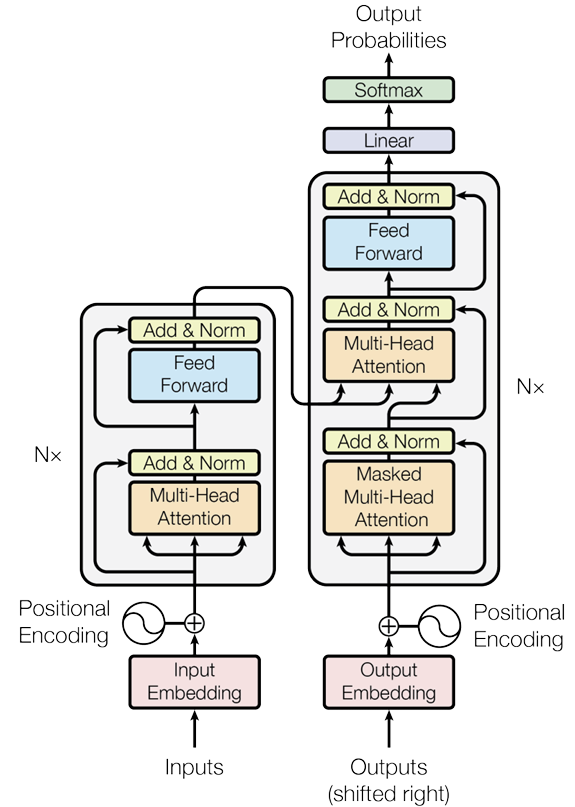
\includegraphics[width=0.55\linewidth]{figures/transformer_Vaswani.png}
\caption[Transformer architecture]{The Transformer architecture, consisting of stacked encoder (left) and decoder (right) blocks. Each encoder layer comprises multi-head self-attention and a feed-forward network with residual connections and layer normalization. The decoder additionally includes masked self-attention to enforce causality and cross-attention over encoder outputs. Adapted from \citet{vaswani2017attention}.}
\label{fig:transformer-architecture}
\end{figure}

Training typically uses \emph{teacher forcing}: at position \(t\), the model is given the ground-truth prefix \(x_{<t}\) and is optimised to assign high probability to the next token \(x_t\). Concretely, parameters are learned by minimizing the negative log-likelihood (equivalently, cross-entropy) over a corpus,
\[
\mathcal{L}=-\sum_{t=1}^{T}\log P\bigl(x_t\mid x_{<t}\bigr).
\]
The architectural mechanism that enforces this conditional structure inside the Transformer is \emph{masked} self-attention: a causal (typically lower-triangular) attention mask prevents each position from attending to any future tokens \(x_{>t}\), ensuring that information flows only from past to present.

This yields an autoregressive factorization of the sequence likelihood:
\[
P(x_{1:T})=\prod_{t=1}^{T}P(x_t\mid x_{<t}),
\]
and generation proceeds one token at a time, conditioning strictly on previously produced tokens; once a token is emitted it becomes part of the immutable context for subsequent predictions.

\begin{figure}[H]
\centering

\includegraphics[width=0.75\linewidth]{figures/background_LLM_images_stanford_CME_Cheatsheet/variants_2_decoder_only.png}
\caption[Decoder-only LLM architecture]{Decoder-only LLMs stack masked self-attention blocks and predict the next token via a linear layer and softmax. Reproduced (cropped) from \citet{amidi2025cme295cheatsheet}, used under the MIT License.}
\label{fig:llm-decoder-only}
\end{figure}

\paragraph{Decoding strategies.} For fixed parameters and fixed context, the forward pass produces a deterministic next-token distribution via a softmax over logits. Apparent stochasticity in model outputs arises primarily from \emph{decoding}: sampling from this distribution using choices such as temperature scaling, top-\(k\) truncation, or nucleus (top-\(p\)) sampling \cite{holtzman2020curiouscaseneuraltext}. Consequently, repeated generations with identical prompts can vary, and controlling the sampling strategy is a key lever for trading off diversity versus determinism.

\begin{figure}[H]
\centering

\includegraphics[width=\linewidth]{figures/background_LLM_images_stanford_CME_Cheatsheet/decoding_sampling_2.png}
\caption[Temperature scaling]{Temperature scaling reshapes the next-token distribution: low \(T\) concentrates probability mass (more deterministic), while high \(T\) flattens it (more diverse). Reproduced (cropped) from \citet{amidi2025cme295cheatsheet}, used under the MIT License.}
\label{fig:llm-temperature}
\end{figure}

\paragraph{Autoregressive generation and hallucination mechanisms.} Modern LLMs generate text through an \textit{autoregressive} language modelling process: tokens are generated sequentially, conditioned on a context \(c\) (e.g., the prompt and any provided documents), such that the probability of a token sequence \(x_{1:T}\) factorizes as:
\begin{equation}
P(x_{1:T} \mid c) = \prod_{t=1}^{T} P(x_t \mid x_{<t}, c)
\end{equation}
At each generation step, the model produces a probability distribution over its vocabulary \(\mathcal{V}\), and a next token is sampled from this distribution. For vocabulary item \(v\in\mathcal{V}\) with logit \(s_v\), the corresponding probability is given by the softmax:
\begin{equation}
P(v \mid x_{<t}, c) = \frac{\exp(s_v)}{\sum_{j \in \mathcal{V}} \exp(s_j)}
\end{equation}
where \(\{s_j\}_{j\in\mathcal{V}}\) are the model's logits for the next-token distribution at step \(t\).

This sequential, generation process has structural properties that contribute to hallucination \citep{ji2023survey}:

\paragraph{Hallucination snowballing.} A form of error propagation that occurs once an incorrect token is generated, the model conditions subsequent generation on this error, compounding inaccuracy. \citet{zhang2023language} demonstrated that LLM hallucinations can ``snowball'' - an initial minor error leads the model to generate increasingly confident but fabricated content to maintain coherence with its erroneous premise. This creates a failure mode where the model appears fluent and confident while being factually wrong.

\paragraph{Decoding-induced degeneration.} The choice of decoding strategy affects hallucination rates. \citet{holtzman2020curiouscaseneuraltext} showed that maximization-based decoding (beam search) can lead to repetitive, degenerate text, while sampling from the full distribution introduces randomness that may select low-probability but plausible-sounding tokens - potentially hallucinations. This tension between coherence and diversity is inherent to autoregressive generation.

Three key parameters control the sampling process:
\begin{itemize}[noitemsep]
    \item \textbf{Temperature} ($T$): Scales logits before softmax, with \(P(v) \propto \exp(s_v / T)\). Lower temperatures ($T < 1$) sharpen the distribution toward high-probability tokens, increasing determinism but risking repetition. Higher temperatures ($T > 1$) flatten the distribution, increasing diversity but also the probability of sampling unlikely (potentially hallucinated) tokens.
    \item \textbf{Top-$k$ sampling}: Restricts sampling to the $k$ highest-probability tokens, redistributing probability mass among them. This prevents sampling from the long tail of implausible tokens, but a fixed $k$ may be too restrictive for peaked distributions or too permissive for flat ones. Therefore, nucleus sampling is often used over top-$k$ for its dynamic properties.
    \item \textbf{Top-$p$ (nucleus) sampling}: Dynamically selects the smallest set of tokens whose cumulative probability exceeds threshold $p$ (e.g., $p=0.9$). This adapts to the shape of each distribution - sampling from few tokens when the model is confident, more when uncertain \citep{holtzman2020curiouscaseneuraltext}.
\end{itemize}
Each parameter represents a trade-off: more restrictive settings reduce hallucination risk but may produce less natural text, while more permissive settings increase fluency at the cost of factual reliability.

\FloatBarrier